\myheader{Guía 2: Caracterización de un Sistema}

\begin{ejercicio}
    Para el sistema en tiempo continuo definido por 
    \begin{align*}
        \inciso y(t) = e^{-t} x(t) & \hfill & \inciso y(t) = 2x(t) + \cos(2t)
    \end{align*}
    se pide:

    \subinciso Determinar si el sistema es lineal.

    \subinciso Encontrar la respuesta del sistema a $x(t)=\delta(t-t_0)$ para cualquier $t_0\in \mathbb{R}$. ¿El sistema es LTI?
    
    \subinciso Decidir si es posible obtener cualquier respuesta del sistema a partir de la respuesta a $x(t)=\delta(t-t_0)$.
\end{ejercicio}
    
\begin{ejercicio}
    Dar, si es posible, un ejemplo de un sistema en tiempo continuo en donde conocer la respuesta a $x(n)=\delta(n-n_0)$ para todo $n_0\in \Z$ no sea suficiente para encontrar la salida del sistema para cualquier $x(n)$.
\end{ejercicio}
    
\begin{ejercicio}
    Para los siguientes sistemas de tiempo continuo
    \begin{align*}
        \inciso y(t) = x(t/3) & \hfill & \inciso y(t) = \int_{-\infty}^{t} x(\tau + 2) d\tau & \hfill & \inciso y(t) = 2x(t) + 1
    \end{align*}
    determinar si cada uno de ellos es lineal, invariante ante desplazamientos, estable, causal y si tiene memoria.
\end{ejercicio}
    
\begin{ejercicio}
    Para los siguientes sistemas de tiempo discreto
    \begin{align*}
        \inciso & y(n) = x(-n) & \hfill \inciso & y(n) = \begin{cases}
        1 & \mbox{para $n = 0$} \\
        \pi x(n) & \mbox{en otro caso}
        \end{cases} \\[.5em]
        \inciso & y(n) = n x(n) & \hfill \inciso & y(n) = \Realpart{x(n)}
    \end{align*}
    determinar si cada uno de ellos es lineal, invariante ante desplazamientos, estable, causal y si tiene memoria.
\end{ejercicio}
    
\begin{ejercicio}
    Calcular $x(n) * x(n)$ con $x(n)=u(n+3) - u(n-4)$.
\end{ejercicio}
    
\begin{ejercicio}
    Dado un sistema LTI cuya respuesta impulsiva está dada por un pulso triangular $h(n)=\delta(n+2)+2\delta(n+1)+3\delta(t)+2\delta(t-1)+\delta(t-2)$ al cual se le aplica una entrada $x(n)$ que consiste en un tren de impulsos de período $N$, calcular y graficar la salida $y(n)$ para los siguientes casos:
    \begin{align*}
    \inciso N=6 & \hfill & \inciso N=4 & \hfill & \inciso N=2
    \end{align*}
\end{ejercicio}
    
\begin{ejercicio}
    A un sistema LTI cuya respuesta al impulso es $h(t) = u(t) - u(t - 1)$ se le aplica una entrada $x(t) = h(t/\alpha)$.
    
    \inciso Calcular la salida del sistema
    
    \inciso Si se sabe que la derivada de la salida tiene sólo 3 discontinuidades, obtener el valor de $\alpha$.
\end{ejercicio}

\begin{ejercicio}
    Dado un sistema LTI en tiempo discreto con una respuesta al impulso $h(n) = \alpha^n u(n)$ con $\alpha<1$, encontrar la salida del sistema para cada una de las siguientes entradas:
    
    \inciso $x(n) = \delta(n) - \delta(n-1)$
    
    \inciso $x(n) = u(n) - u(n-5)$
\end{ejercicio}
    
\begin{ejercicio}
    Dado un sistema LTI en tiempo continuo, encontrar la salida del sistema cuando la entrada es $x(t) = u(t-1)\sin(t)$ si la respuesta al impulso es:
    
    \inciso $h(t) = u(n)$ 
    
    \inciso $h(t) = u(t) - 2u(t-2) + u(t-5)$
\end{ejercicio}

\begin{ejercicio}
    Sobre un único sistema invariante en el tiempo se conocen los siguientes pares entrada-salida:
    \begin{align*}
        x_1(n) = \delta(n) + 2\delta(n-2) & \hspace{1em}\longrightarrow\hspace{1em} y_1(n) = \delta(n-1) + 2\delta(n-2) \\[.5em]
        x_2(n) = 3 \delta(n-2) & \hspace{1em}\longrightarrow\hspace{1em} y_2(n) = \delta(n-1) + 2 \delta(n-3) \\[.5em]
        x_3(n) = \delta(n-3) & \hspace{1em}\longrightarrow\hspace{1em} y_3(n) = \delta(n+1) + 2 \delta(n) + \delta(n-1)
    \end{align*}
    
    \inciso ¿Se puede afirmar algo sobre la linearidad del sistema?
    
    \inciso ¿Es posible hallar la respuesta del sistema $y_4(n)$ cuando la entrada es $x_4(n)=\delta(n)$ con los datos disponibles? En tal caso, obtenerla.
    
    \inciso ¿Es posible hallar la respuesta del sistema $y_5(n)$ cuando la entrada es $x_5(n)=5\delta(n-2)$ con los datos disponibles? En tal caso, obtenerla.
\end{ejercicio}

\begin{ejercicio}
    Determinar si los siguientes enunciados son verdaderos o falsos.
    
    \inciso La conexión en cascada de sistemas LTI resulta en un sistema total que también es LTI.
    
    \inciso La conexión en cascada de sistemas no lineales es un sistema no lineal.
    
    \inciso La conexión en cascada de sistemas no invariantes en el tiempo es un sistema no invariante en el tiempo.
    
    \inciso La conexión en cascada de sistemas causales con sistemas causales es siempre no causal.
    
    \inciso El orden de conexión de sistemas no invariantes en el tiempo no altera la salida para una misma entrada.
    
    \inciso En un sistema LTI si la entrada es periódica entonces la salida también lo es.
\end{ejercicio}
    
\begin{ejercicio}
    Dos sistemas LTI en tiempo discreto con respuesta al impulso $h_1(n)$ y $h_2(n)$ son conectados en cascada en ese orden. La entrada no se conoce pero la salida $y(n)$ es como se muestra en la siguiente figura:
    \begin{center}
        \begin{tikzpicture}[scale=0.6,transform shape]
    \begin{axis}[
        x=0.1\textwidth,y=0.1\textwidth,
    	axis y line=center,
    	axis x line=middle,
    	xlabel=$n$,ylabel={\LARGE $x(n)$},
    	xmin=-7.5,xmax=7.5,
    	ymin=-1.3,ymax=2.9,
    	xticklabel style = {xshift=0},
    	yticklabel style = {yshift=5},
    	]
    	\discretedelta{-7}{0.1};
    	\discretedelta{-6}{0.1};
    	\discretedelta{-5}{0.1};
    	\discretedelta{-4}{0.1};
    	\discretedelta{-3}{0.1};
    	\discretedelta{-2}{0.1};
    	\discretedelta{-1}{1};
    	\discretedelta{0}{2};
    	\discretedelta{1}{-1};
    	\discretedelta{2}{1};
    	\discretedelta{3}{0.1};
    	\discretedelta{4}{0.1};
    	\discretedelta{5}{0.1};
    	\discretedelta{6}{0.1};
    	\discretedelta{7}{0.1};
    \end{axis}
\end{tikzpicture}
    \end{center}
    
    \inciso Si los dos sistemas son causales, ¿qué se puede decir acerca del momento en que la entrada podría haber empezado? ¿Se puede establecer el momento exacto de comienzo?
    
    \inciso La entrada $x(n)$ que produjo la salida $y(n)$ anterior es aplicada a un nuevo par de sistemas conectados en cascada donde el primero tiene una respuesta impulsiva $h_a(n) = h_1(n + 1)$ y el segundo $h_b(n) = 2h_2(n)$. Graficar la salida.
\end{ejercicio}
    
\begin{ejercicio}
    En el sistema de la figura se sabe que $\gamma \in \Z_{\geq 0}$ y $\beta, \alpha_1, \alpha_2 \in \R$ con $\alpha_1 \neq \alpha_2$.
    \begin{center}
        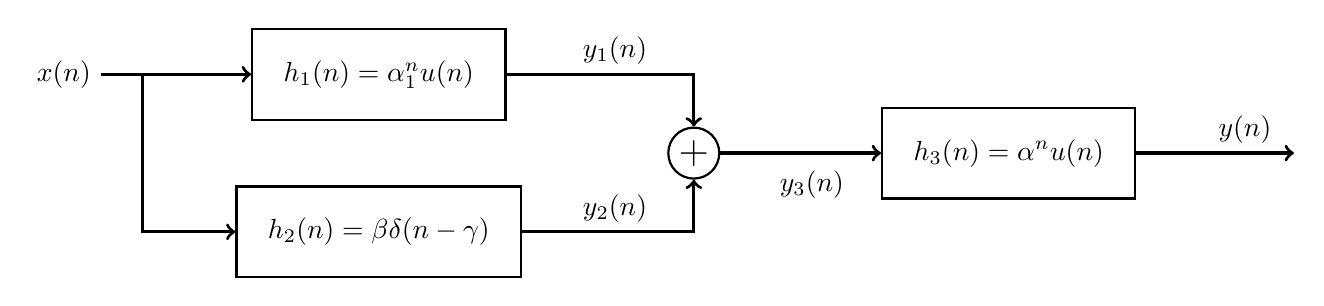
\begin{tikzpicture}
    \node[circle,draw,thick,inner sep=0.05cm] (plus) at (0,0) {\Large +} ;
    \node[rectangle,draw,thick,inner sep=0.4cm] (h1) at (-4,1) {$h_1(n)=\alpha_1^n u(n)$} ;
    \node[rectangle,draw,thick,inner sep=0.4cm] (h2) at (-4,-1) {$h_2(n)=\beta \delta(n-\gamma)$} ;
    \node[rectangle,draw,thick,inner sep=0.4cm] (h3) at (4,0) {$h_3(n)=\alpha^n u(n)$} ;
    \node[xshift=-4cm] (x_n) at (h1) {$x(n)$} ;
    \node[xshift=-3cm,inner sep=-0.1] (x_n_arrow_cross) at (h1) {} ;

    \node[xshift=3cm,yshift=.3cm] (y_1) at (h1) {$y_1(n)$} ;
    \node[xshift=3cm,yshift=.3cm] (y_2) at (h2) {$y_2(n)$} ;
    \node[xshift=-2.5cm,yshift=-.4cm] (y_3) at (h3) {$y_3(n)$} ;
    \node[xshift=3cm,yshift=.3cm] (y_n) at (h3) {$y(n)$} ;

    \draw[->, very thick] (x_n) -- (h1.west) ;
    \draw[->, very thick] (x_n_arrow_cross) |- (h2.west) ;
    \draw[->, very thick] (h1.east) -| (plus.north) ;
    \draw[->, very thick] (h2.east) -| (plus.south) ;
    \draw[->, very thick] (plus.east) -- (h3.west) ;
    \draw[->, very thick] (h3.east) -- ++(2,0) ;
\end{tikzpicture}
    \end{center}

    \inciso Determinar $h(n)$ tal que $y(n) = h(n) * x(n)$.

    \inciso Determinar las condiciones que deben cumplir los parámetros $\alpha_1, \alpha_2, \beta, \gamma$ para que el sistema sea estable.
\end{ejercicio}

\begin{ejercicio}
    Dado un sistema LTI con $h(t) = u(t + T/2) - u(t - T/2)$ donde $T>0$, se desea analizar cómo el sistema opera sobre señales periódicas.
    
    \inciso Demostrar que para cualquier señal periódica de período $T$ la salida es constante para todo $t$.

    \inciso Determinar el valor de la constante si se sabe que la señal periódica es impar.

    \inciso Determinar si existen señales periódicas de período $T'\neq T$ para las cuales los resultados anteriores siguen siendo ciertos.
\end{ejercicio}

\begin{ejercicio}
    Sea un sistema LTI y una señal $x(n)$ que satisface $x(n)=\delta(n) + \sum_{k=1}^M a_k x(n-k)$ donde $a_k$ son valores reales. Sea $y(n)$ la salida del sistema para la entrada $x(n)$.

    \inciso Determinar la ecuación en diferencias de $h(n)$ en función de $y(n)$ usando las propiedades básicas de los sitemas LTI.
    
    \inciso Si $y(n)$ es de duración finita, ¿qué se puede decir sobre la estabilidad del sistema?

    \inciso Si $y(n)$ es de duración infinita, obtener algún tipo de condición sobre $y(n)$ que asegure la estabilidad del sistema.
\end{ejercicio}

\begin{ejercicio}
    Sea un sistema LTI de tiempo discreto tal que la relación entre la salida y la entrada del mismo se puede escribir como:
    \begin{equation*}
        y(n) = \sum_{k=0}^{\infty} \alpha^{n-k} \left(x(k) + \beta x(k-1) + \gamma x(k-2)\right)
    \end{equation*}
    donde $|\alpha| < 1$ y $\beta, \gamma \in \R$.

    \inciso Obtener la respuesta al impulso del sistema y graficarla.
    \inciso Analizar la estabilidad del mismo.
    \inciso Determinar los valores de $\beta$ y $\gamma$ para que el sistema tenga las siguientes propiedades:
    \begin{itemize}
        \item Si $x(n) = (-1)^n$ para todo $n$ entonces $y(n) = 0$ para todo $n$.
        \item Si $x(n) = 1$ para todo $n$ entonces $y(n) = 1$ para todo $n$.
    \end{itemize}
\end{ejercicio}

\begin{ejercicio}
    Dado un sistema en tiempo discreto definido por la ecuación en diferencias 
    \begin{equation*}
        y(n) = x(n) + \frac{3}{4} y(n-1)
    \end{equation*}
    con condiciones de contorno
    \begin{align*}
    \inciso & y(-1) = 0 & \inciso & y(1) = 0 & \inciso & y(0) = 0 \\[.5em]
    \inciso & y(0) = 1 & \inciso & \lim_{n\rightarrow -\infty} y(n) = 0  & \inciso & \lim_{n\rightarrow +\infty} y(n) = 0
    \end{align*}
    se pide:
    \begin{itemize}
        \item Calcular el valor de la respuesta al impulso $h(n)$ del sistema en el intervalo $-5 \leq n \leq 5$
        \item Obtener una expresión cerrada de $h(n)$ para todo $n \in \mathbb{Z}$.
        \item Determinar si el sistema lineales, invariante ante desplazamientos, estables y causales.
    \end{itemize}
\end{ejercicio}
    
\begin{ejercicio}

    Dado un sistema en tiempo discreto definido por la ecuación en diferencias 
    \begin{equation*}
        y(n) = x(n) + \frac{1}{2} y(n-1)
    \end{equation*}
    con condiciones
    
    \inciso iniciales de reposo

    \inciso finales de reposo

    \noindent se pide:
    \begin{itemize}
        \item Determinar si el sistema lineales, invariante ante desplazamientos, estables y causales. Establecer cómo se relacionan las condiciones de contorno con cada una de las propiedades del sistema.
        \item Calcular el valor de la respuesta a las señales $\delta(n-1)$ y $\delta(n+1)$ del sistema en el intervalo $-5 \leq n \leq 5$.
        \item Obtener una expresión cerrada de la respuesta a las señales $\delta(n-1)$ y $\delta(n+1)$ para todo $n \in \mathbb{Z}$.
    \end{itemize}
\end{ejercicio}
    
\begin{ejercicio}
    Demostrar que un sistema definido por ecuaciones en diferencias FIR siempre será lineal, invariante ante desplazamientos y estable. Determinar, además, qué condición debe cumplir un sistema de este tipo para ser causal.
\end{ejercicio}
    
\begin{ejercicio}
    Obtener la respuesta al impulso para el sistema definido por la ecuación diferencial 
    \begin{equation*}
        y(n) = x(n+1) + x(n) + x(n-1) + \frac{3}{4} y(n-1)
    \end{equation*}
    en condiciones inciales de reposo. 
\end{ejercicio}
    
\begin{ejercicio}
    Obtener la respuesta al impulso para el sistema definido por la ecuación diferencial 
    \begin{equation*}
        y(n) = x(n+1) + x(n) + x(n-1) + \frac{5}{4} y(n-1)
    \end{equation*}
    en condiciones finales de reposo. 
\end{ejercicio}
    
\begin{ejercicio}
    Implementar en \Keyboardsym una función que permita obtener la respuesta al impulso de una ecuación en diferencias para condiciones iniciales o finales de reposo.
\end{ejercicio}
    
    
    